\documentclass{article}

% \usepackage[spanish]{babel}

\usepackage[utf8]{inputenc}
\usepackage{graphicx}

\title{Ecuaciones en diferencias}

\author{Alumnos de 3er semestre grupo 2}

\date{18 de septiembre de 2017}

\begin{document}

\maketitle

\section{Ecuaciones de primer orden}

\subsection{Ecuaciones lineales}

Una ecuación lineal en diferencias de primer orden tiene la forma $x_{n+1}=ax_n$ donde $a$ es una constante. 

La fórmula para resolver ecuaciones lineales es:
\begin{equation}
  \label{lineal}
  x_n=a^nx_0
\end{equation}

Por ejemplo, si inciamos una inversión con 1000 pesos con un interés mensual del 1\%, obtenemos lo siguiente:

\begin{center}
  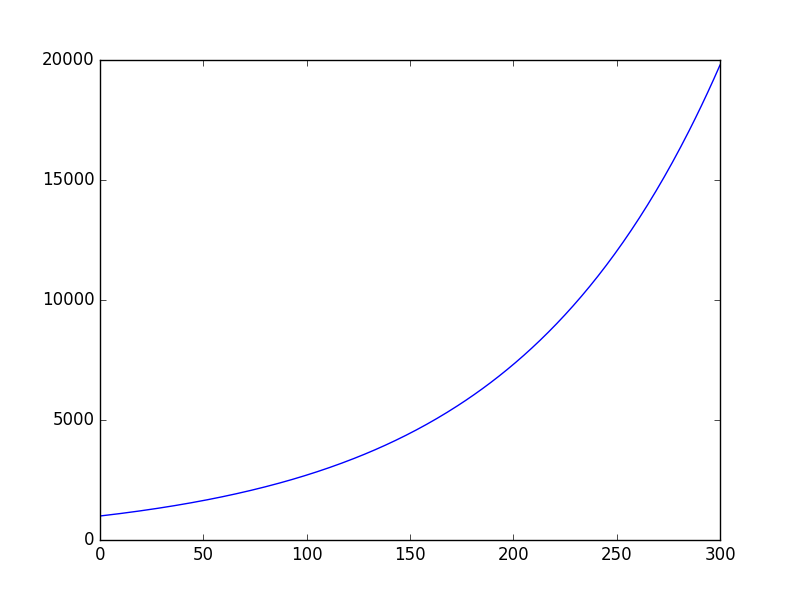
\includegraphics[width=8cm]{inversion.png}
\end{center}

\subsection{Ecuaciones afines}

Una ecuación afín en diferencias de primer orden tiene la forma $x_{n+1}=ax_n+b$ donde $a$ es una constante. 

\begin{equation}
  \label{afin}
  x_n=a^n(x_0-\alpha)+\alpha
\end{equation}

donde $\alpha=\frac{b}{1-a}$. 

Para deducir esta fórmula usamos que $$\sum_{i=0}^{n-1}a^i=\frac{a^n-1}{a-1}$$.

\subsection{Ejemplito}

Nuestro compañerito Pepe muere en raras circunstancias, luego descubren lo radiante de su ser. cada 20 años el elemento radioactivo decae a razón de $2%$, si inicialmente contenía 2 kilitos de puro amor ¿Cuánto tendrá cuando se vea un poco más feo (como quien digo, dentro de 200 años)?
\section{Ecuaciones de segundo orden}

El método para resolver estas ecuaciones está inspirado en la fórmula \ref{lineal}.

Para resolver una ecuación en diferencias de segundo orden se usa la ecuación resolvente.

Una ecuación en diferencias de segundo orden , tiene la forma $a_{k+2}=f(a_k ,a_{k+2}$
Esta ecuaci\'on no tiene raices reales $$x^2+1=0$$
\end{document}